\section{Use-Case Analysis and Design} \label{sec:usecase}

\subsection{Use Case}
This sector defines the functional requirements for the app. In summary, the app has \textbf{1 actor} and \textbf{10 use cases}. An actor models a type of role played by an entity that interacts with the app. The actor can be a human user or an external system. Meanwhile, a use case describes a sequence of interactions between actors and systems to accomplish a particular goal. Use cases are usually referred to as system functionalities that a system should perform in interaction with one or more external users (actors). In the case of the thesis, the actor is the users, and the system is the mobile application. The figure below is the proposed UML \cite{uml} use case diagram: \par

\begin{figure} [H]
    \centering
    \captionsetup{justification=centering}
    \includegraphics[width=1.0\textwidth]{chapter3/image/use-case.png}
    \caption{Use case diagram for the hair and clothes app}
    \label{fig:schnet_LiNet}
\end{figure}

With each use case, it is accompanied by a table describing it. In tables, the "Pre-condition" row is a list of conditions that must be met before the action of that use case. The "Post-condition" row is a list of conditions that must be reached after the action of that use case. The "Expected result" row lists acceptable results of that use case.

\begin{center} 
\begin{table} [H]
\caption{Hair camera use-case description} 
\begin{tabular}{p{0.35\linewidth} | p{0.6\linewidth}}
\hline
USER CASE            & UC-1 \\ \hline
Use case name        & Hair Camera   \\ \hline
Use case description & Real-time camera preview with hair \\ \hline
Pre-condition         &   User were in the app's main screen, selected the “Hair Camera” option. Request permissions must be accepted before camera starts \\ \hline
Post-condition        &   Camera preview is displayed in response to the hardware. Hair mask is overlayed directly on frames  \\ \hline
Basic flow           &   \begin{enumerate}
    \item User switches front to rear camera, and vice versa.
    \item User changes color of hair.
    \item User clicks the capture button.
\end{enumerate}   \\ \hline
Alternate flows      &   \begin{enumerate}
    \setcounter{enumi}{3}
    \item User clicks the back button
\end{enumerate}   \\ \hline
Expected result      &  \begin{enumerate}
    \item If permissions are not granted, ask for the permissions.
\end{enumerate}    \\ \hline
\end{tabular}
\end{table}
\end{center}


\begin{center}
\begin{table} [H]
\caption{Clothes camera use-case description} 
\begin{tabular}{p{0.35\linewidth} | p{0.6\linewidth}}
\hline
USER CASE            & UC-2 \\ \hline
Use case name        & Clothes Camera  \\ \hline
Use case description & Real-time camera preview with clothes recolored     \\ \hline
Pre-condition         &   User were in the app's main screen, selected the “Clothes Camera” option. Request permissions must be accepted before camera starts   \\ \hline
Post-condition        &   Camera preview is displayed in response to the hardware. Clothes mask is directly overlaied on frames   \\ \hline
Basic flow           &  \begin{enumerate}
  \item Users switch front to rear camera, and vice versa.
  \item Users change color for clothes.
  \item	Users click the capture button. 
\end{enumerate} \\ \hline
Alternate flows      &   \begin{enumerate}
    \setcounter{enumi}{3}
    \item User clicks the back button, returning to the main screen
\end{enumerate}   \\ \hline
Expected result      &  \begin{enumerate}
    \item If permissions are not granted, ask for the permissions
\end{enumerate}    \\ \hline
\end{tabular}
\end{table}
\end{center}


\begin{center}
\begin{table} [H]
\caption{Change lens use-case description} 
\begin{tabular}{p{0.35\linewidth} | p{0.6\linewidth}}
\hline
USER CASE            & UC-3 \\ \hline
Use case name        &  Change lens  \\ \hline
Use case description &   One button is responsible for switching between front and rear lens  \\ \hline
Pre-condition         &   Camera preview is displayed, but user want to the other camera instead   \\ \hline
Post-condition        &   Preferable camera lens is chosen. User is now ready for capture.   \\ \hline
Basic flow           &  \begin{enumerate}
  \item User clicks on lens switching button.
  \item	Preview camera displays image for the front camera if the rear camera is opening. 
  \item New mask is generated and replaces the old one.
\end{enumerate}    \\ \hline
Alternate flows      &   N/A   \\ \hline
Expected result      & \begin{enumerate}
    \item User is able to change between camera lenses multiple times.
\end{enumerate}     \\ \hline
\end{tabular}
\end{table}
\end{center}


\begin{center}
\begin{table} [H]
\caption{Capture use-case description} 
\begin{tabular}{p{0.35\linewidth} | p{0.6\linewidth}}
\hline
USER CASE            & UC-4 \\ \hline
Use case name        &  Capture \\ \hline
Use case description &  One button is responsible for capture from camera     \\\hline
Pre-condition         &   Camera preview is displayed, user switched to lens his/her want. Now, user want to capture the frame at that moment  \\ \hline
Post-condition        &   Frame is captured and ready for latter use  \\ \hline
Basic flow           &   \begin{enumerate}
    \item 	User clicks on capture button
\item Stop camera previewing
\item The frame at the moment is saved to memory
\item Show options to treat the captured frame
\end{enumerate}
\\ \hline
Alternate flows      & N/A     \\ \hline
Expected result      &  
\begin{enumerate}
    \item User is able to capture multiple times.
\end{enumerate}   \\ \hline
\end{tabular}
\end{table}
\end{center}


\begin{center}
\begin{table} [H]
\caption{Clothes segmentation use-case description} 
\begin{tabular}{p{0.35\linewidth} | p{0.6\linewidth}}
\hline
USER CASE            & UC-5 \\ \hline
Use case name        &  Clothes segmentation  \\ \hline
Use case description &  Clothes color in a chosen image is recolored    \\\hline
Pre-condition         &   User was in the app’s main screen, selected the “Clothes segmentation” option. Permission requests must be accepted before camera starts   \\ \hline
Post-condition        &   Input image is recolored and applied filter. User gets recolored image his/her want.   \\ \hline
Basic flow           &   \begin{enumerate}
    \item Choose an image from gallary
\item Choose color for clothes in image
\item Choose filter that is going to apply to the image
\item Save \& Share the new image
\end{enumerate}
   \\ \hline
Alternate flows      &    \begin{enumerate}
    \setcounter{enumi}{4}
    \item User clicks on Back button, return to the main screen
\end{enumerate}  \\ \hline
Expected result      &  \begin{enumerate}
    \item If user chooses unsupported file format, showing up this error
\item New image is saved and shared successfully
\end{enumerate}    \\ \hline
\end{tabular}
\end{table}
\end{center}

%finish

\begin{center}
\begin{table} [H]
\caption{Hair segmentation use-case description} 
\begin{tabular}{p{0.35\linewidth} | p{0.6\linewidth}}
\hline
USER CASE            & UC-6 \\ \hline
Use case name        &  Hair segmentation  \\ \hline
Use case description &  Hair color in a chosen image is recolored    \\\hline
Pre-condition         &   User was in the app’s main screen, selected the “Hair segmentation” option. Permission requests must be accepted before camera starts   \\ \hline
Post-condition        &   Input image is recolored and applied filter. User gets recolored image his/her want.   \\ \hline
Basic flow           &   \begin{enumerate}
    \item Choose an image from gallary
    \item Choose color for hair in image
    \item Choose filter that is going to apply to the image
    \item Save \& Share the new image
\end{enumerate}
   \\ \hline
Alternate flows      &    \begin{enumerate}
    \setcounter{enumi}{4}
    \item User clicks on Back button, return to the main screen
\end{enumerate}  \\ \hline
Expected result      &  \begin{enumerate}
    \item 	If user chooses unsupported file format, showing up this error
    \item 	New image is saved or shared successfully
\end{enumerate}    \\ \hline
\end{tabular}
\end{table}
\end{center}

\begin{center}
\begin{table} [H]
\caption{Hair color scanning use-case description} 
\begin{tabular}{p{0.35\linewidth} | p{0.6\linewidth}}
\hline
USER CASE            & UC-7 \\ \hline
Use case name        &  Hair color scanning  \\ \hline
Use case description &  Hair color on camera preview will continuously switch to all colors.    \\\hline
Pre-condition         &  User was in the app’s main screen, selected the “Hair color scanning” option. Permission requests must be accepted before camera starts    \\ \hline
Post-condition        &   User looked at his/her hair in different colors. User want to experience other user cases.   \\ \hline
Basic flow           &  \begin{enumerate}
    \item Camera opens, switching camera lens as user want
\item	Hair mask renders directly on camera preview

\end{enumerate}    \\ \hline
Alternate flows      &   \begin{enumerate}
    \setcounter{enumi}{2}
    \item User clicks on Back button, return to the main screen
\end{enumerate}   \\ \hline
Expected result      &  \begin{enumerate}
    \item Hair is recolored successfully
    \item User is able to change camera lens
\end{enumerate}    \\ \hline
\end{tabular}
\end{table}
\end{center}

\begin{center}
\begin{table} [H]
\caption{Select color use-case description} 
\begin{tabular}{p{0.35\linewidth} | p{0.6\linewidth}}
\hline
USER CASE            & UC-8 \\ \hline
Use case name        &  Select color  \\ \hline
Use case description &   User can select a color from color palette for mask. Hair or clothes would be changed to that color at once   \\\hline
Pre-condition         &   User are at preview camera with mask overlaid, but he/she want to change mask to a different color   \\ \hline
Post-condition        &   User chose his/her favorite color and come back to preview camera    \\ \hline
Basic flow           &  \begin{enumerate}
    \item 	User clicks on the color palette button
\item	A color palette shows up 
\item User clicks on the color his/her like
\item The color palette disappears, return to camera preview screen
\end{enumerate}    \\ \hline
Alternate flows      &   N/A   \\ \hline
Expected result      &  \begin{enumerate}
    \item 	If the chosen color is different with previous color, change mask’s color
\item If the color palette button is clicked in the second times, color palette disappears.
\end{enumerate}    \\ \hline
\end{tabular}
\end{table}
\end{center}

%finish

\begin{center} 
\begin{table} [H]
\caption{Apply filter use-case description} 
\begin{tabular}{p{0.35\linewidth} | p{0.6\linewidth}}
\hline
USER CASE            & UC-9 \\ \hline
Use case name        &  Apply filter  \\ \hline
Use case description &  Filters that is listed for user to edit image    \\\hline
Pre-condition         &   User after recoloring hair or clothes wants to edit the image more  \\ \hline
Post-condition        &   User finishes editting   \\ \hline
Basic flow           &  \begin{enumerate}
    \item Show filters available 
    \item User chooses an filter
    \item Preview image after apply filter
    \item User accept the filter
\end{enumerate}    \\ \hline
Alternate flows      &   N/A   \\ \hline
Expected result      &  \begin{enumerate}
    \item If user refuses to apply filter, image stayes the same
\end{enumerate}     \\ \hline
\end{tabular}
\end{table}
\end{center}

\begin{center} 
\begin{table} [H]
\caption{Save \& Share use-case description} 
\begin{tabular}{p{0.35\linewidth} | p{0.6\linewidth}}
\hline
USER CASE            & UC-10 \\ \hline
Use case name        &  Save \& Share  \\ \hline
Use case description &   Each image that is taken before, is opted to delete or save or share   \\\hline
Pre-condition         &   User clicked capture button   \\ \hline
Post-condition        &  Photograph is saved/shared and user want to take another    \\ \hline
Basic flow           &   \begin{enumerate}

    \item Show images that is captured before
    \item User clicks onto save button
    \item Image is saved into storage
    \item User clicks onto share button
    \item User choose where to share the image
    \item Return to preview camera screen
\end{enumerate}   \\ \hline
Alternate flows      &  \begin{enumerate}
    \setcounter{enumi}{6}
    \item User clicks back button, then return to preview camera screen
\end{enumerate}    \\ \hline
Expected result      &   
\begin{enumerate}
    \item An image can be both saved and shared
\end{enumerate}  \\ \hline
\end{tabular}
\end{table}
\end{center}

\subsection{Sequence Diagram}

In this phase, we are going to discuss diagrams showing the interactions between objects in the app, arranged
in a sequence. These following diagrams also show a series of messages exchanged by objects that perform a specific task or action. Clothes Camera and Hair Segmentation use cases are chosen to elaborate with sequence diagrams, as these use cases are representative and substantial in the app.  

\begin{figure}[H]
    \centering
    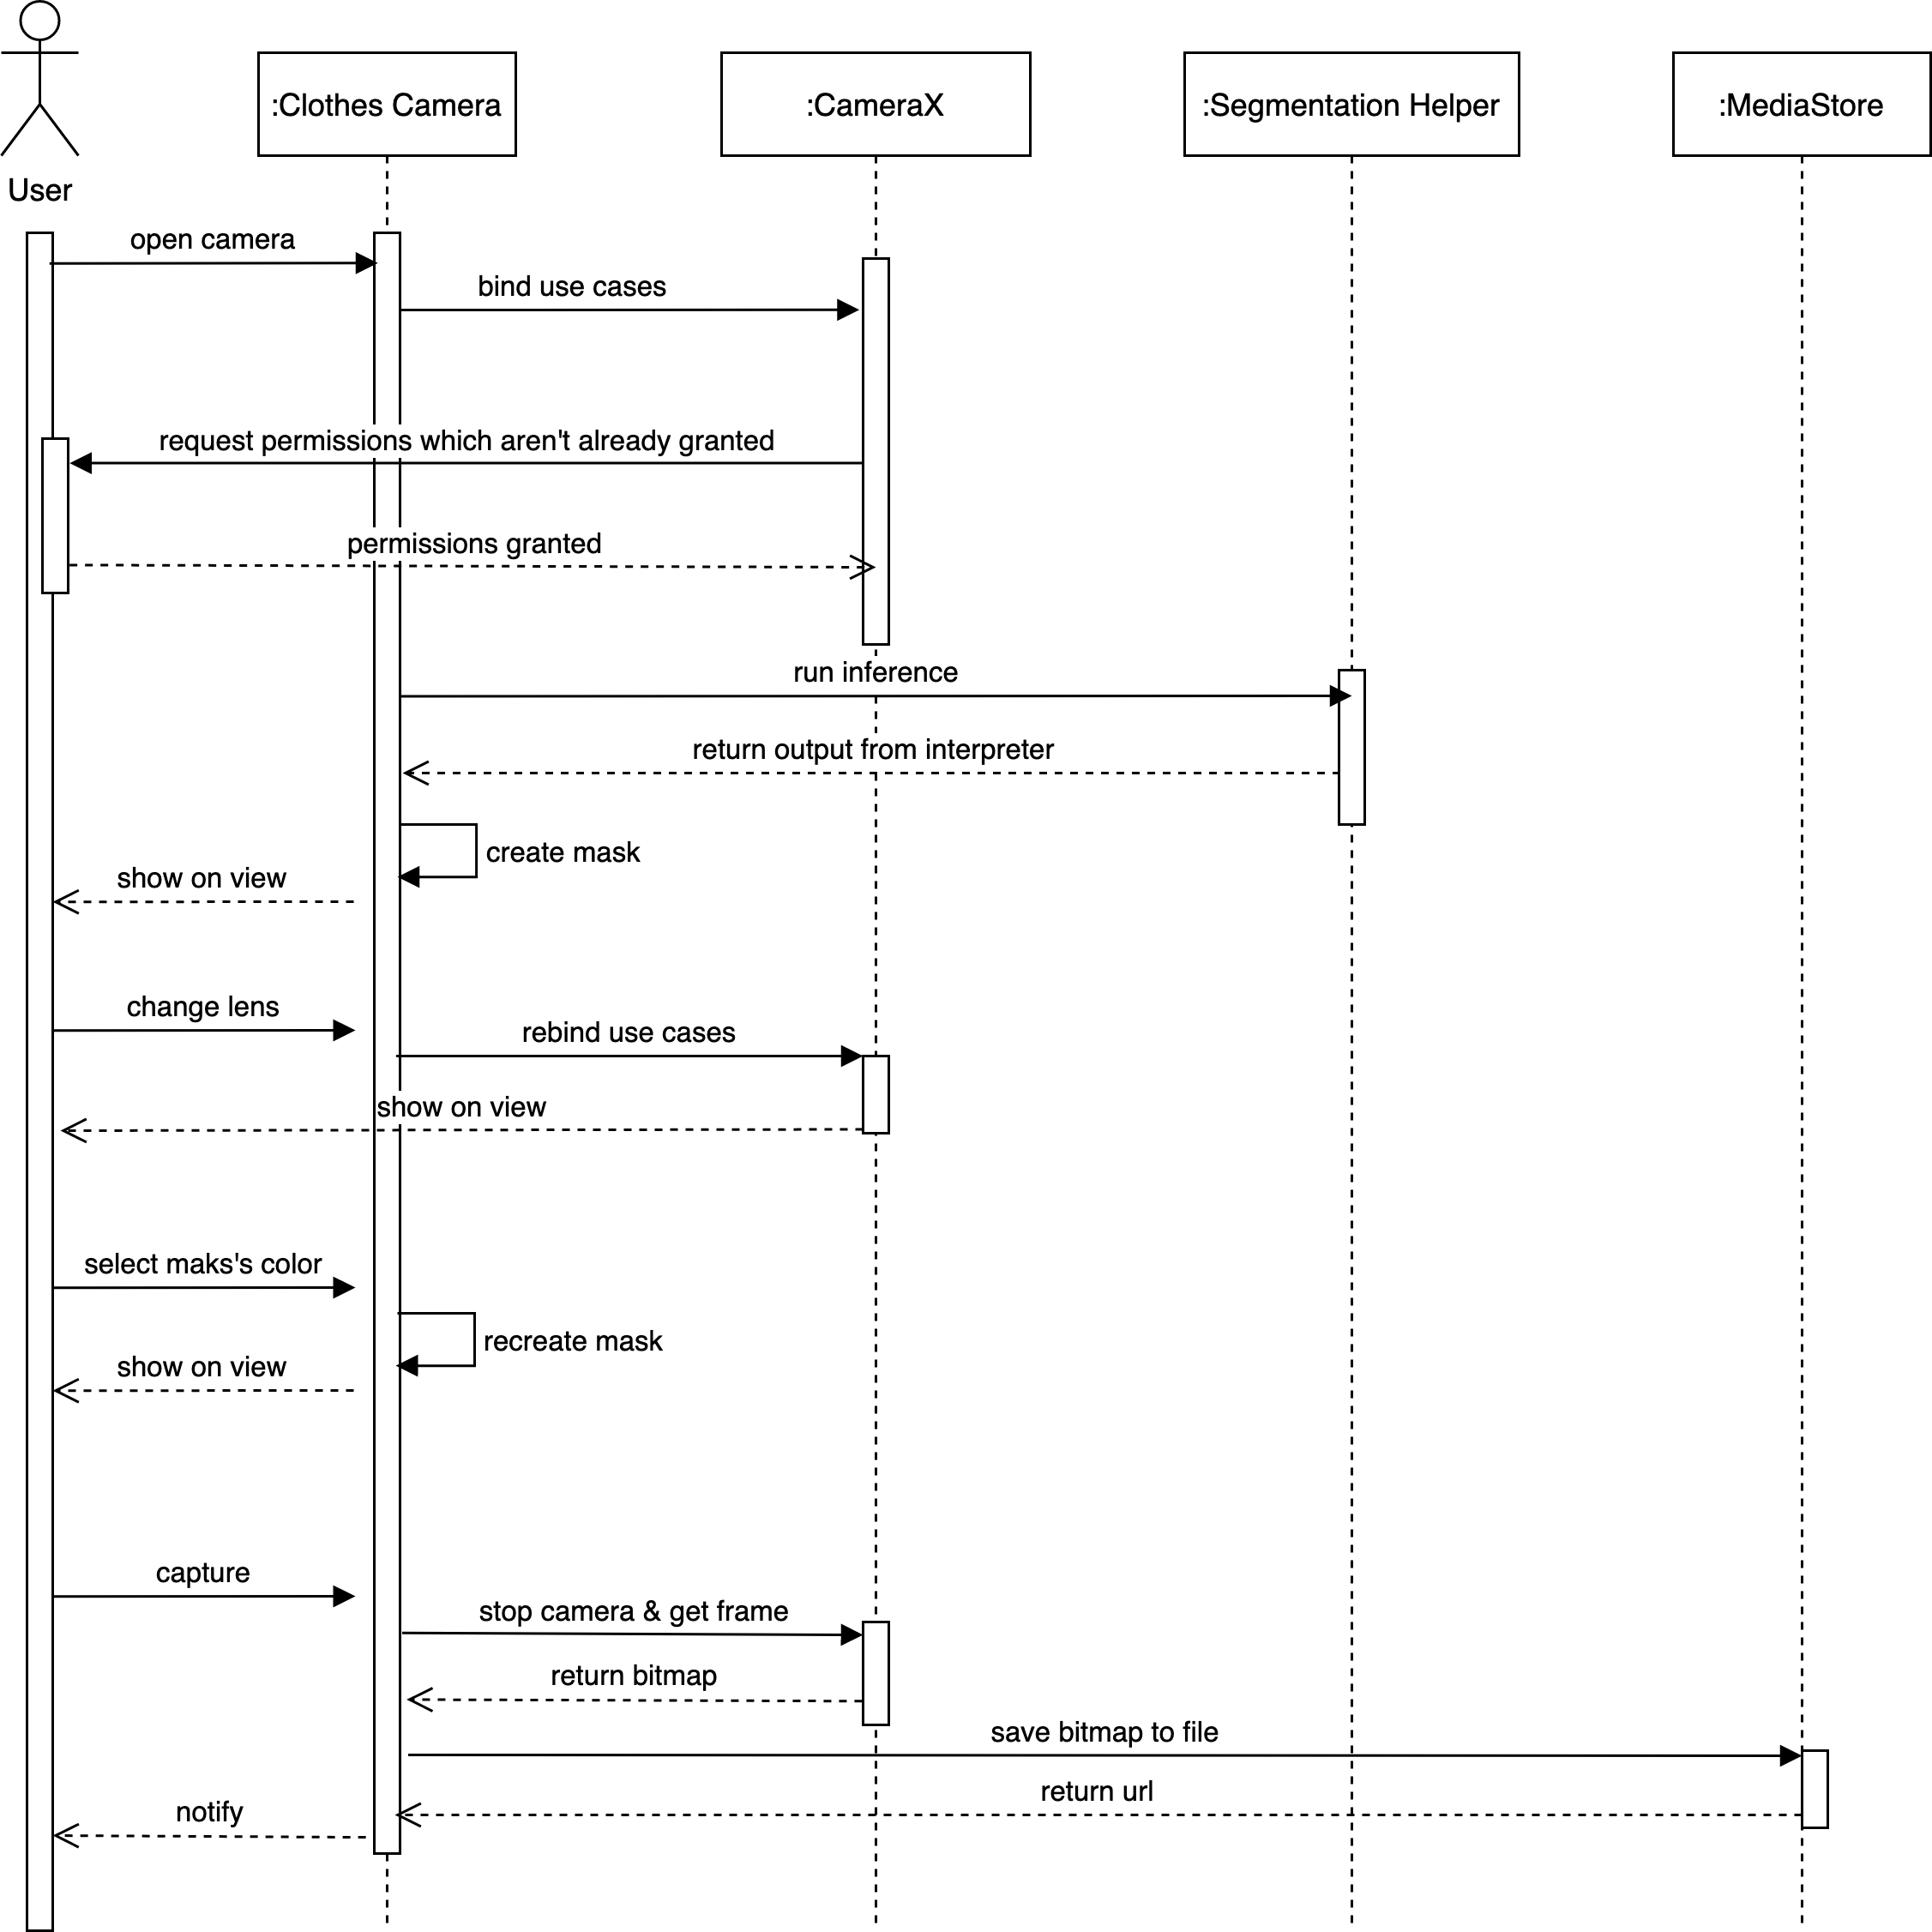
\includegraphics[width=1.0\textwidth]{chapter3/image/clothescamera.png}
    \caption{Sequence diagram for Clothes Camera use case}
    \label{fig:my_label}
\end{figure}

\begin{figure}[H]
    \centering
    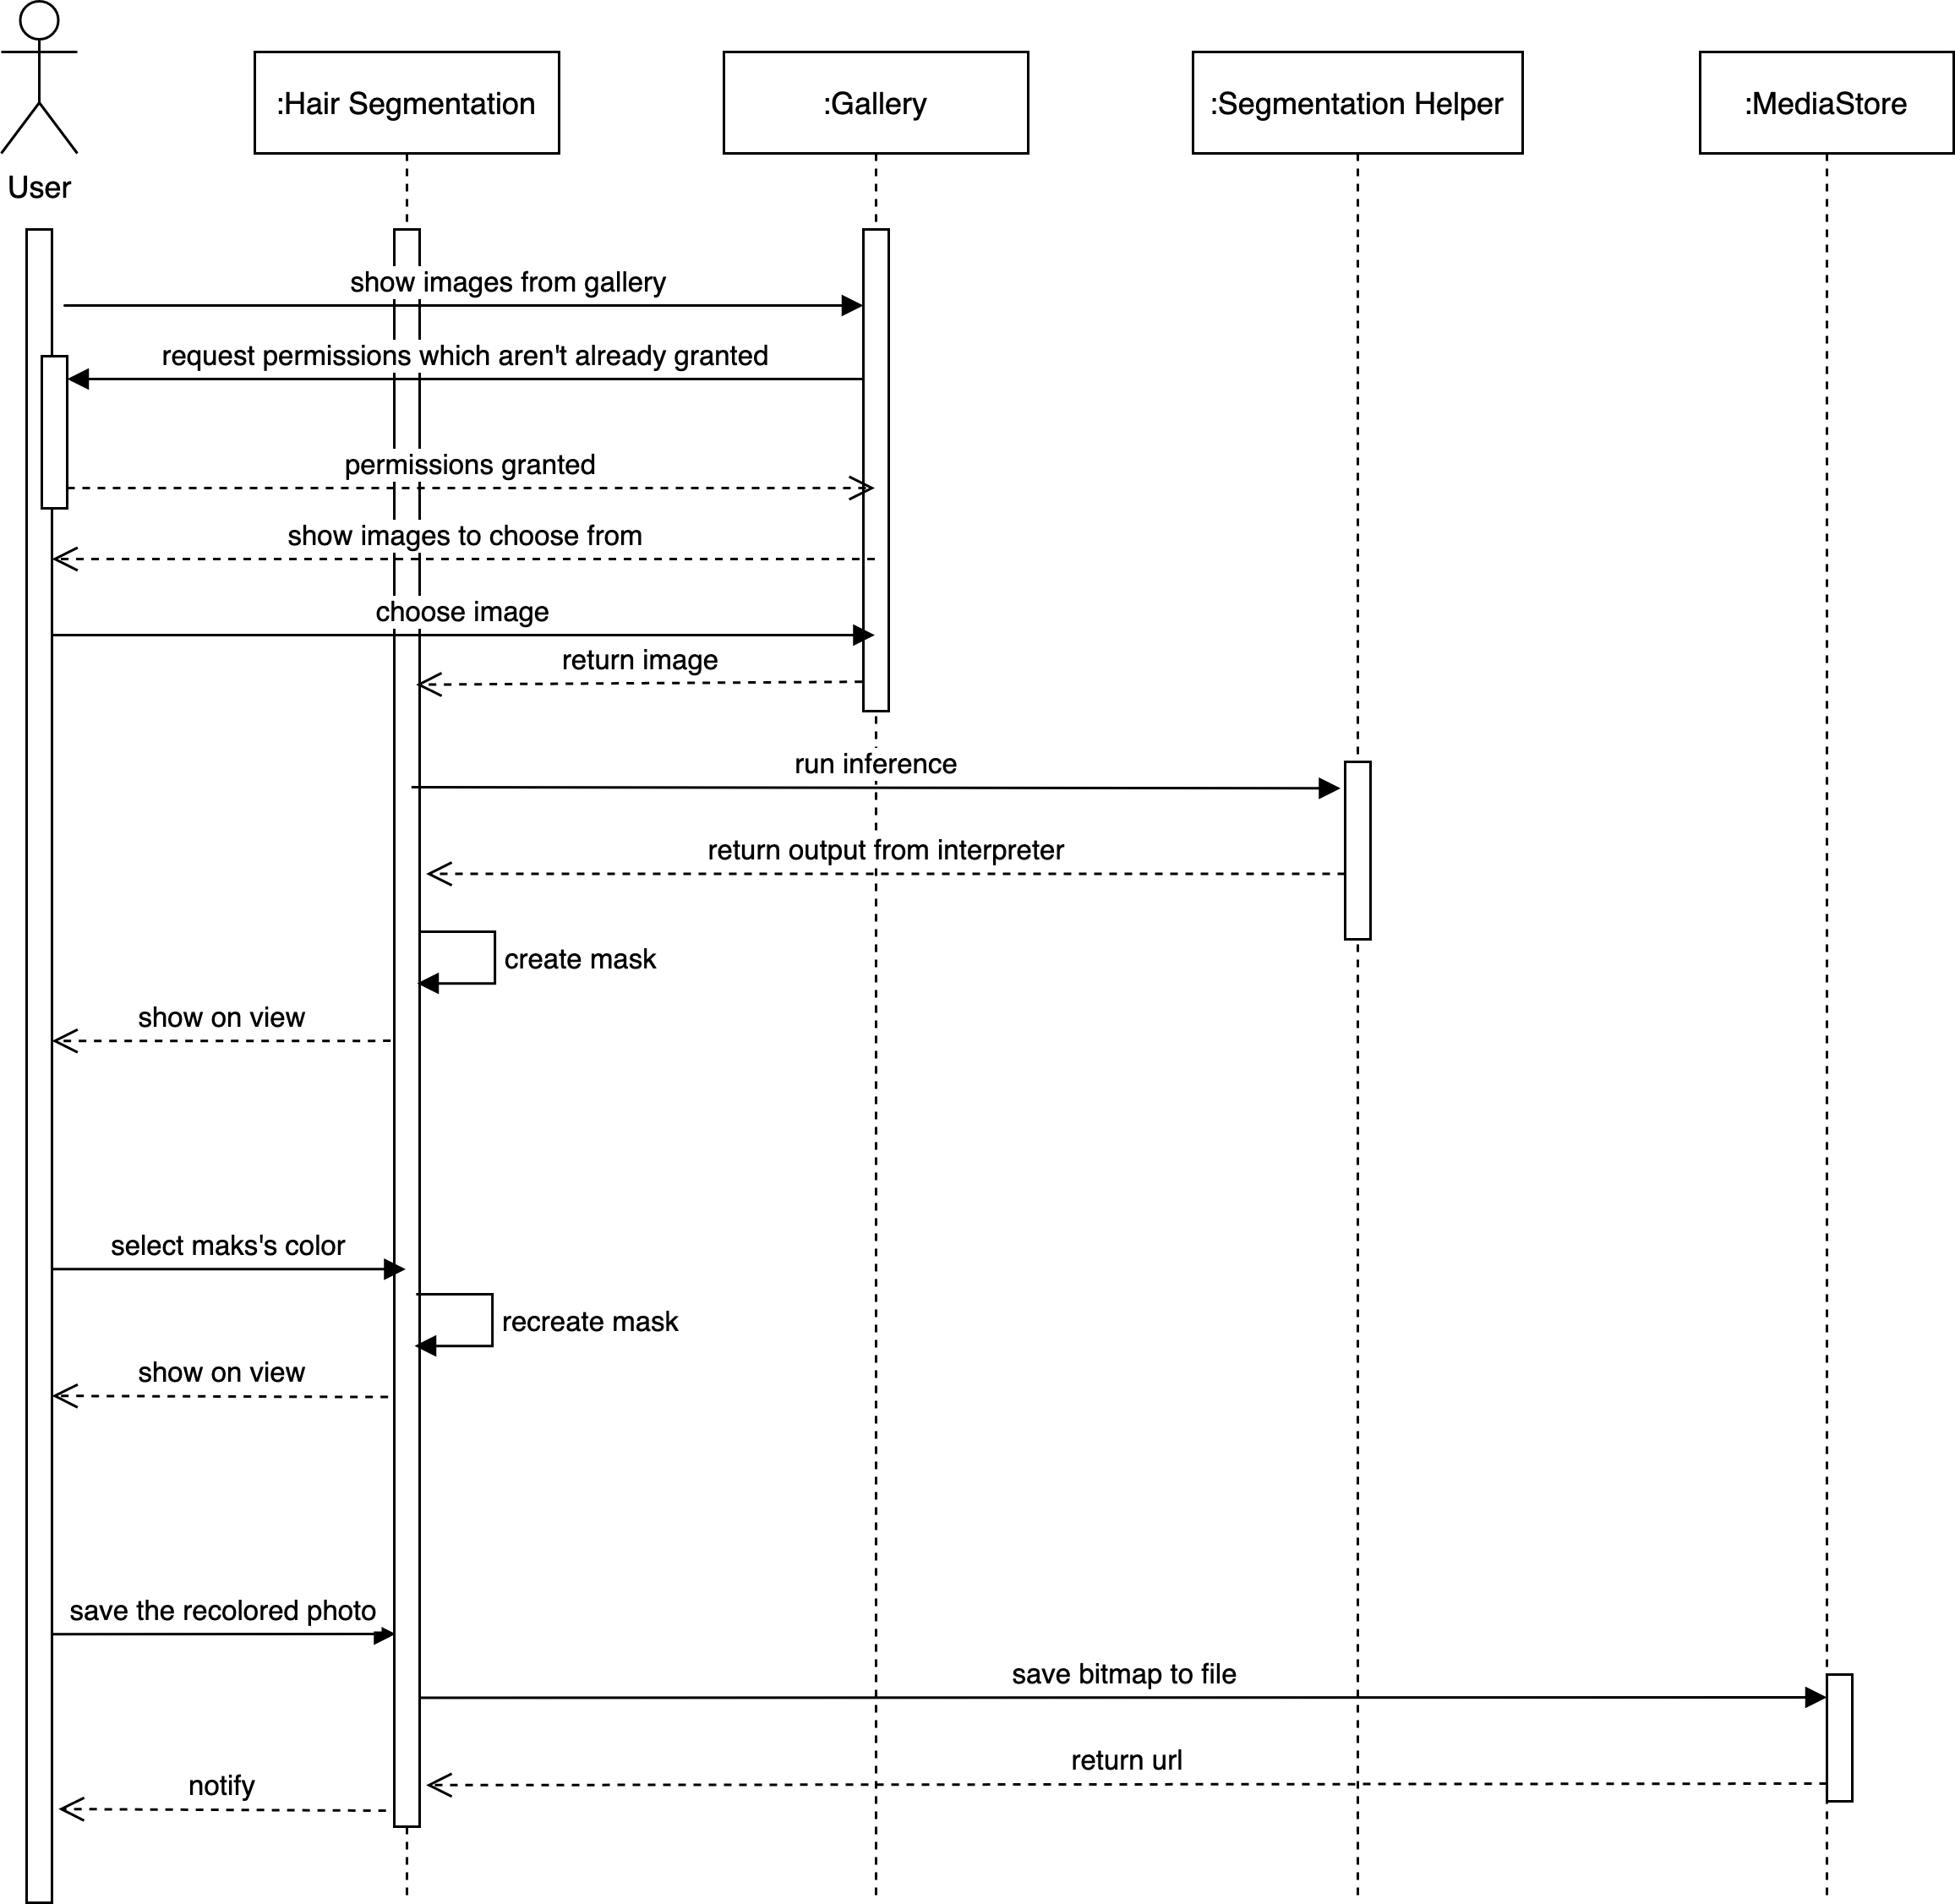
\includegraphics[width=1.0\textwidth]{chapter3/image/hairsegmentation.png}
    \caption{Sequence diagram for Hair Segmentation use case}
    \label{fig:my_label}
\end{figure}
